% Created 2024-12-02 Mon 10:12
% Intended LaTeX compiler: pdflatex

% BEGIN
% Classe du document et encodage
% --------------------------------------------------
\documentclass[12pt]{article}
\usepackage[utf8]{inputenc}                    % Standard UTF-8
\usepackage[T1]{fontenc}                       % Standard UTF-8
\usepackage{natbib}
\setcitestyle{super}
\bibpunct{(}{)}{,}{a}{}{}
\usepackage[francais, english]{babel}
\usepackage{times}

% Disposition du document
% --------------------------------------------------
\usepackage[left=2.5cm,right=2.5cm,top=2.5cm,bottom=2.5cm]{geometry}
\usepackage[pagestyles]{titlesec}
\usepackage{hyperref}
\usepackage[title]{appendix}
\usepackage{setspace}
\newpagestyle{main}{\setfoot{}{}{\thepage}}
\pagestyle{main}

% Symboles mathématiques et notation diverse
% --------------------------------------------------
\usepackage{amsmath,amssymb,mathrsfs,nicefrac,esint}
\usepackage{xparse,physics}
\usepackage{color,soul}
\usepackage{verbatim}
\usepackage{textcomp}
\usepackage{lipsum}
\numberwithin{equation}{section}

% Nouvelles notations
\newcommand{\HRule}{\rule{\linewidth}{0.5mm}}
\newcommand{\dash}[0]{\,\text{-}\,}
\newcommand*\circled[1]{\tikz[baseline=char.base)]{
    \node[shape=circle,draw,inner sep=2pt] (char) {#1};
}}
\newcommand{\mcb}[2]{\colorbox{#1}{$\displaystyle #2$}}
\DeclareMathOperator{\sinc}{sinc}
\DeclareMathOperator{\PPCM}{PPCM}
\DeclareMathOperator{\e}{e}
\DeclareMathOperator{\del}{\partial}

% Commandes des environnements mathématiques
\newcommand{\aeq}[1]{\begin{align}#1\end{align}}
\newcommand{\aeqn}[1]{\begin{align*}#1\end{align}}
\newcommand{\hfrac}[2]{\nicefrac{#1}{#2}}
\newcommand{\siunit}[1]{\mathrm{[#1]}}
\newcommand{\sifunit}[2]{\mathrm{[\nicefrac{\mathrm{#1}}{\mathrm{#2}}]}}
\newcommand{\evaluate}[2]{\left.#1\right|_{#2}}
\newcommand{\sgn}[1]{\mathrm{sgn}\qty(#1)}

% Listes et tableaux
% --------------------------------------------------
\usepackage{array,booktabs,multirow,colortbl,tabularx}
\usepackage[shortlabels]{enumitem}
\numberwithin{table}{section}
\renewcommand{\arraystretch}{1.2}

% Environnement des figures et animations
% --------------------------------------------------
\usepackage{graphicx,float,subcaption}
\usepackage{chngpage}
\usepackage[space]{grffile}
\usepackage{tikz,animate,pgf}
\usetikzlibrary{
    arrows,backgrounds,calc,patterns,positioning,shapes.geometric,babel,shadows,
    shadings,decorations.pathmorphing,shapes.misc
}
\graphicspath{{Figures/}}
\numberwithin{figure}{section}

% Références
% --------------------------------------------------
\usepackage[nottoc,notlof,notlot]{tocbibind}
\usepackage{url}
\bibliographystyle{abbrvnat-fr}

% ================================SETTINGS=================================%
% Pas d'indentation en début de paragraphe :
%\setlength\parindent{0pt}
%\setlength{\parskip}{0.15cm}
% Couleur references
\definecolor{hrefcol}{RGB}{147,0,255}
\definecolor{tcorange}{RGB}{255,165,0}
\definecolor{tcyellow}{RGB}{255,255,150}
\hypersetup{colorlinks,
             filecolor=hrefcol,
             urlcolor=hrefcol,
             citecolor=hrefcol,
             linkcolor=hrefcol,
             anchorcolor=hrefcol}

\usepackage[utf8]{inputenc}
\usepackage[T1]{fontenc}
\usepackage{graphicx}
\usepackage{grffile}
\usepackage{longtable}
\usepackage{wrapfig}
\usepackage{rotating}
\usepackage[normalem]{ulem}
\usepackage{amsmath}
\usepackage{textcomp}
\usepackage{amssymb}
\usepackage{capt-of}
\usepackage{hyperref}
\graphicspath{{Figures/}}
\author{Xavier Chartrand}
\date{02-12-2024}
\title{Présentation des données de vagues AZMP}
\hypersetup{
 pdfauthor={Xavier Chartrand},
 pdftitle={Présentation des données de vagues AZMP},
 pdfkeywords={},
 pdfsubject={},
 pdfcreator={Emacs 27.1 (Org mode 9.3)}, 
 pdflang={English}}
\begin{document}

\maketitle
\tableofcontents


\section{Réseau AZMP}
\label{sec:orgc1fd6bc}
\begin{figure}[H]
\centering
\makebox[\textwidth][c]{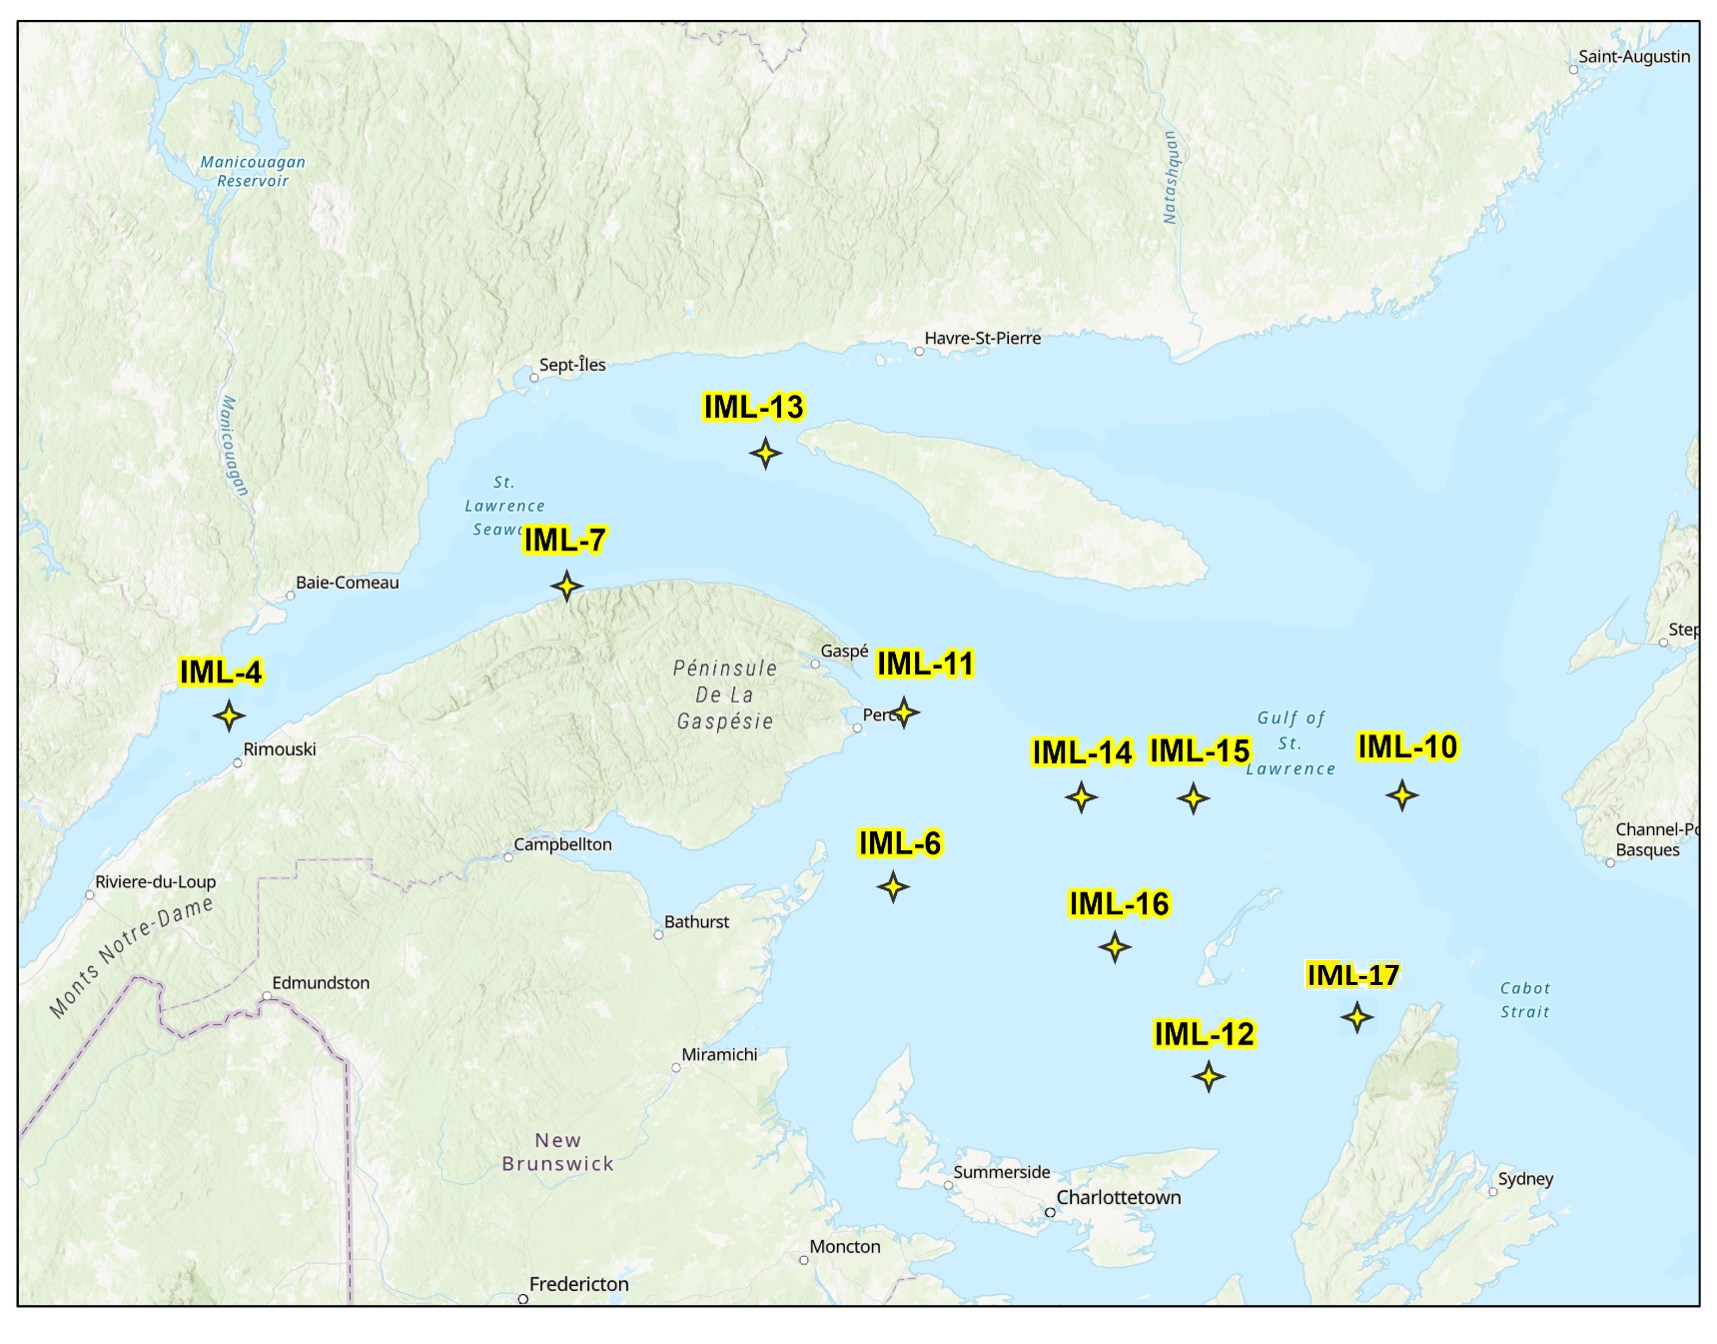
\includegraphics[width=44pc]{Figures/reseau_azmp.png}}
\caption{}
\end{figure}

\begin{itemize}
\item Bouées de vague (IML-4-6-7-10-11-12-14) \\
\item Hydrophones (IML-13-15-16-17)
\end{itemize}

\section{Traitement des données}
\label{sec:org71bb02a}
\subsection{Ancien contrôleur}
\label{sec:org8a81260}
L'ancien contrôleur comprend l'ensemble des bouées avant 2023. En 2023, un
nouveau contrôleur a été installée sur la bouée IML-4, et pour les années à
suivre. Ce nouveau contrôleur sera installée sur les bouées IML-11 et
AZMP-STA27 en 2024. Éventuellement, le MPO vise à installer ce nouveau
contrôleur sur l'ensemble des bouées du réseau.

L'ancien et le nouveau contrôleur ont des similitudes, mais ils ne mesurent
pas le champ de vagues de la même façon. Les deux utilisent le même moniteur
de vagues qui consistent en un accéléromètre trois axes installé sur la
bouée. Aucune correction n'est apportée aux accélérations pour prendre en
compte ses mouvements rotatoires autour de ses trois axes. La correction doit
être faite séparément, à l'aide de données fournies par un compas séparément
monté sur le contrôleur. L'ancienne version utilise le compas XX et la
nouvelle, le compas YY
\%
\subsection{Champ de vagues IML-4 2023}
\label{sec:orgf74c980}
Hauteur significative versus amplitude du vent
\begin{figure}[H]
\centering
\makebox[\textwidth][c]{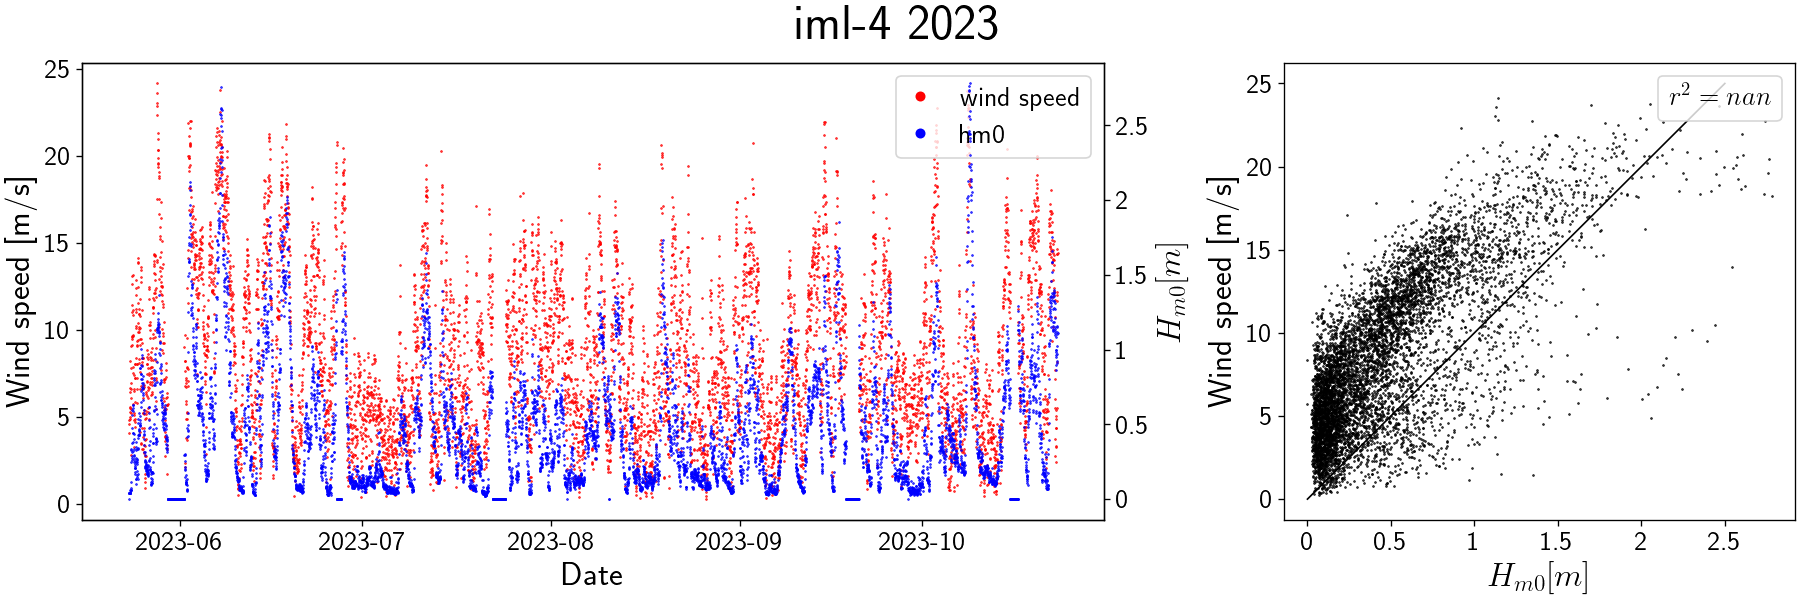
\includegraphics[width=44pc]{Figures/windwave_magnitude_iml-4_2023.png}}
\end{figure} ~\\[12pt]
%
Direction des vagues versus direction du vent
\begin{figure}[H]
\centering
\makebox[\textwidth][c]{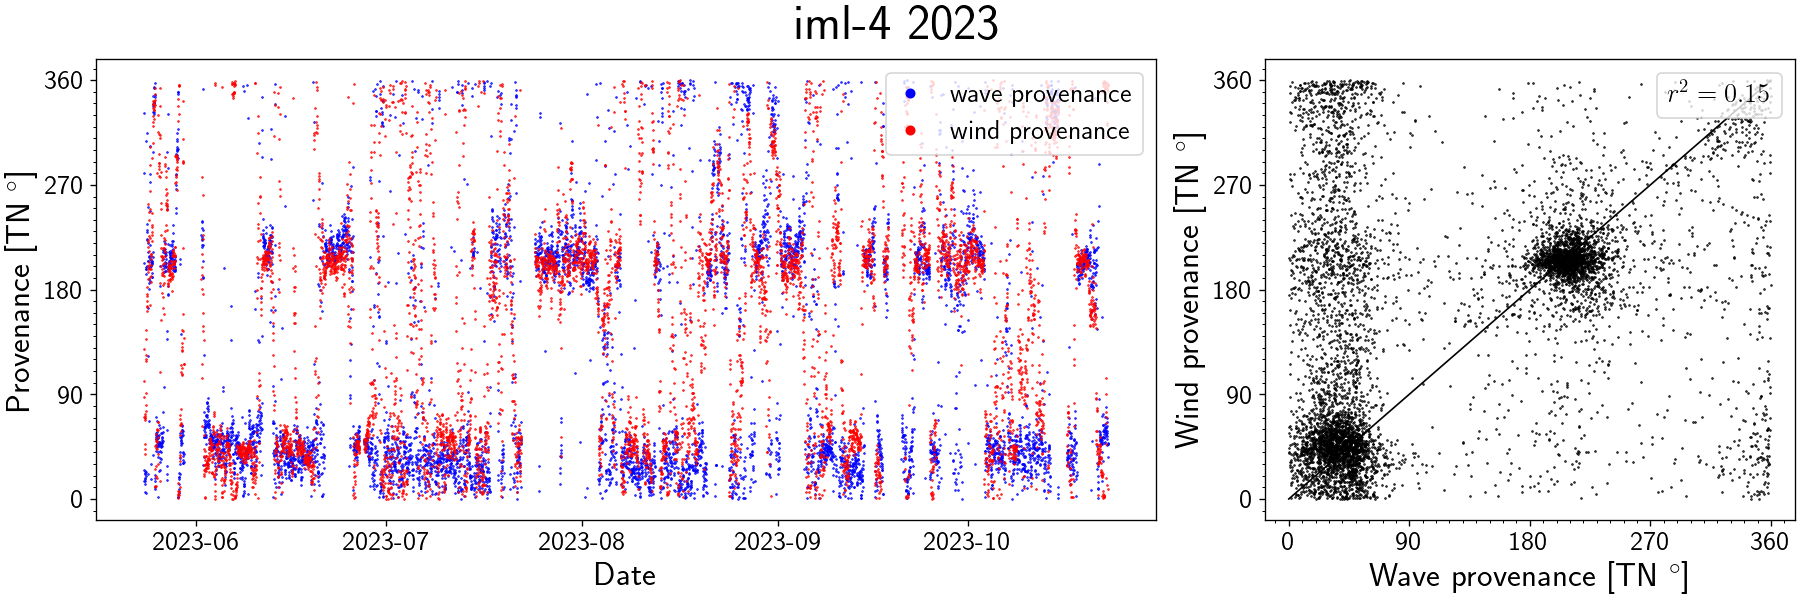
\includegraphics[width=44pc]{Figures/windwave_direction_iml-4_2023.png}}
\end{figure}
\end{document}
